\documentclass{sig-alternate}
\usepackage{color}
\usepackage[colorinlistoftodos]{todonotes}

%%%%% Uncomment the following line and comment out the previous one
%%%%% to remove all comments
%%%%% NOTE: comments still occupy a line even if invisible;
%%%%% Don't write them as a separate paragraph
%\newcommand{\mycomment}[1]{}

\begin{document}

% --- Author Metadata here ---
%%% REMEMBER TO CHANGE THE SEMESTER AND YEAR AS NEEDED
\conferenceinfo{UMM CSci Senior Seminar Conference, April 2017}{Morris, MN}

\title{Convolutional Neural Networks in Medical Imaging}

\numberofauthors{1}

\author{
% The command \alignauthor (no curly braces needed) should
% precede each author name, affiliation/snail-mail address and
% e-mail address. Additionally, tag each line of
% affiliation/address with \affaddr, and tag the
% e-mail address with \email.
\alignauthor
Mitchell Finzel\\
	\affaddr{Division of Science and Mathematics}\\
	\affaddr{University of Minnesota, Morris}\\
	\affaddr{Morris, Minnesota, USA 56267}\\
	\email{finze008@morris.umn.edu}
}

\maketitle
\begin{abstract}
Over the past 5 years there has been an increase in the use of convolutional neural networks in a broad variety of medical imaging applications. This is due in part to the increase in their popularity since their success in the 2012 ImageNet competition, but is also due to their adaptability across a range of medical imaging applications. These applications vary greatly; from the segmentation of knee cartilage to the detection of Alzheimer's disease in MRIs and much more. In this paper we will go over some of the cutting edge architecture techniques being used specifically for the tasks of brain segmentation; classifying with both binary segmentation on brain lesions and hierarchical segmentation with tumors. The results are proving to be quite promising with many of the described techniques outscoring previous state-of-the-art systems.

\end{abstract}

\keywords{ACM proceedings, \LaTeX, text tagging}

\section{Introduction}
\label{sec:introduction}

In 2012 convolutional neural networks or CNNs, were used to great success improving drastically over the previous state-of-the-arts in the ImageNet computer vision competition~\cite{NIPS:2012}. Since their success in image recognition CNNs have seen a rise in popularity, finding their way into more complex computer vision challenges such as medical imaging. In the past 5 years there has been an increase in the use of CNNs in biological segmentation tasks. These tasks extend across a wide variety of human anatomy. For example, CNNs have been used for the automated detection of lymph nodes~\cite{Roth:2014}, the segmentation of knee cartilage~\cite{Prasoon:2013} and Alzheimer's detection ~\cite{Payan:2015} to name a few. For this paper we will be focusing on two specific examples of CNN use in medical imaging segmentation:~\cite{Havaei:2017} by Havaei, et al. and~\cite{Kamnitsas:2017} by Kamnitsas, et al. These two papers show different approaches to CNN architectures applied to the segmentation of MRIs. While the results obtained by both approaches are not directly comparable, we will go through what makes their approaches unique and where there is some overlap. After discussing their features we will take a look at their state-of-the-art results on a few different segmentation challenges.

\begin{figure}
\centering
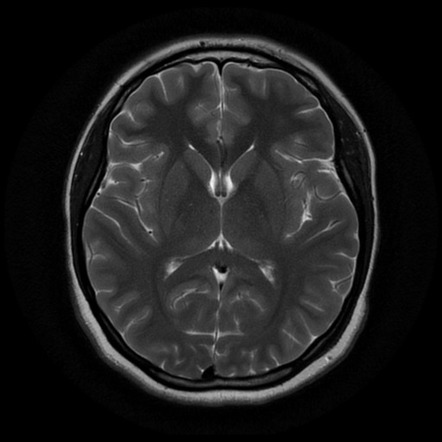
\psfig{file=brainMRI.jpeg,width =3in}
\caption{An MRI of a 'normal' young persons brain. https://radiopaedia.org/cases/normal-brain-mri-3}
\label{fig:brainMRI}
\end{figure}

\section{Background}
\label{sec:background}

Before delving into the specifics of the network architecture approaches that are being employed we will look at some of the fundamentals of CNNs and segmentation in general. When discussing segmentation in the field of medical imaging we are discussing the ability to classify different parts of a medical image. This segmentation is fairly loosely defined and can be used to describe classification through a variety of granularities. On a more course granularity we might have an x-ray of a leg where we desire to differentiate and label the different bones in the image. On a finer granularity we might be interested in being able to identify and label tumors in an MRI of a brain. Currently most of this segmentation is done by hand by medical professionals, this is where convolutionl neural networks come in. The CNN is trained on a set of images that have been properly labeled by medical professionals which teaches it how to differentiate the different parts of the image on its own. The network can then take unlabeled images as input and uses its training to attempt to label the image on its own. The end goal is the network outputting an image that has been properly labeled, much as though it had been labeled by hand. 

\subsection{Introduction to Neural Networks}
\label{sec:introNeuralNetworks}

At their most basic form neural networks are pattern recognizers modeled off of the neuronal structures of the cerebral cortex, the part of the brain that takes in sensory data. The networks are generally comprised of layers of nodes that activate when they recognize a certain input. The result of these activations are then passed to neighboring nodes through weighted connections. After passing   through the layers of nodes and connections the resulting data is sent out of the network as some form of output data. What makes neural networks so powerful is their general usability and their ability to alter the weights of the node connections in response to the accuracy of their output.

In our case we are interested in a type of neural network called a convolutional neural network. CNNs are based on many of the same principals of a normal neural network, but have an additional type of layer that has been found very useful when it comes to learning things about images.

\begin{figure}
\centering
\psfig{file=Neural Network.png,width =3in}
\caption{A simple artificial neural network. https://en.wikipedia.org/wiki/Artificial\_neural\_network}
\label{fig:ANN}
\end{figure}

\subsection{Convolutional Layers}
\label{sec:convolutionalLayers}

Convolutional Layers are what differentiate convolutional neural networks from other neural networks, the first layer of all CNNs is a convolutional one. The convolutional layer takes an array of values that represents either the pixels or voxels of the input image. The layer then uses what is interchangeably called a filter, neuron or kernel, which is another array with the same depth as the input array. The kernel is then aligned to the upper left corner of the input, the area it covers is called the receptive field. The array contained within the receptive field is then multiplied with the array in the kernel using element-wise multiplication. The multiplications are then summed up and stored in the same relative position of what's called a feature map as seen in figure~\ref{fig:ActivationMap}. The kernel then slides over a specified distance on the input and performs the same operation. What we end up with after all of the possible convolutions of the kernel and the input is a completed feature map. The feature map is an array that contains all of the results of the convolutions between the kernel and the input.

\begin{figure}
\centering
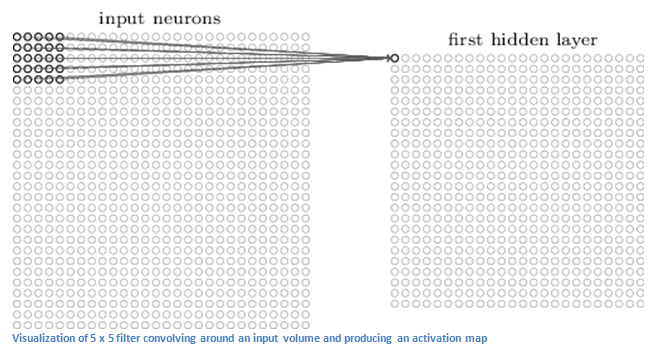
\psfig{file=ActivationMap.png,width =3in}
\caption{Visualization of kernel activations being stored in the feature map, also known as an activation map. https://adeshpande3.github.io/}
\label{fig:ActivationMap}
\end{figure}

\subsection{Kernels}
\label{sec:kernels}

Kernels, as described above, are arrays of values that are meant to represent features to be recognized. For instance a kernel could contain a feature such as a curve. This might be represented by a pattern of numbers in the kernels array. When the kernel is multiplied with the input the result will be a higher number if the feature in the kernel is similar to the feature explained by the receptive field. If the feature described by the kernel is not present in the receptive field then the result of the multiplication will be relatively smaller. These recognitions of features are then stored in the feature map where they will likely be used as the input to the next layer. To increase the depth of feature recognition in a layer, just add more kernels. As these feature maps are used in future layers of similar operations a hierarchy of features is created with more complex features being represented in later layers.

\subsection{Pooling Layers}
\label{sec:poolingLayers}

Another often used layer type is called a pooling layer. These layers have a relatively straightforward purpose, they take clusters from the input feature map and reduce them down to a single feature. For instance, an example of a pooling operation is max-pool. A max-pool pooling layer will divide the input into clusters and place the highest value of each cluster in their corresponding place in the pooling layer's feature map. Pooling layers are used to drastically reduce the amount of spacial data by eliminating a large portion of the input in one step. They also reduce the effects of overfitting, which is essentially when the neural network becomes too finely tuned to the training data and fails to generalize well.

\subsection{Fully Connected Layers}
\label{sec:fullyConnected}

The fully connected layer can be thought of as the final layer in the network. It takes in as input a feature map from the prior layer and returns a vector of probabilities that the input was a certain label. As a medical based example I might have a CNN that is trying to segment what is and isn't a tumor. The output is therefore a binary option, tumor or non-tumor. The fully connected layer looks at the features represented in the feature map and then provides a vector with two values, the probability that the input is a tumor and the probability that it is not a tumor.

\subsection{Training}
\label{sec:training}

Now that we have gone through some of the components of a CNN we can get into the thing that makes it all work, the training process. Before going into the basic steps of the training process it is important to note that a training data set is required to begin the process. The training data set in our case would be medical images that have already been segmented by hand. This way we have images that the network can try to segment and then check its results against the labels provided.

The kernels in the network originally start off randomized and therefore the output probabilities should all be approximately equal. On the forward pass an image patch from the training data is sent through the network and the output probability is compared to the true label probability provided with the test image. This comparison is put through a loss function to quantify the inaccuracy. At the start of the training process the loss will likely be very high with the goal being a loss score representing the predicted labels equivalency of the true label. The loss function is then used in the next step of the process called the backward pass. In the backward pass you progress back through the network, evaluating which kernels contributed the most to the total loss and calculating the weight adjustments that would minimize said loss. After the backward pass is complete the final step, weight update, is performed. This final step takes the loss minimizing weight changes from the backward pass phase and implements them. Applying this four step process for every image in the test data set is considered one epoch; training is generally conducted over many epochs.

After completing the training process the network can be tested on a testing data set. The testing data set much like the training data contains images and their true labels. The data in the testing set cannot contain images from the training set because of the inherent bias the network has towards the images it was trained on.

There are a few things that are important to note when it comes down to the training process. In general the more images in the training data set the better. This can be a hurdle for medical image applications, due to the difficulty of gathering appropriate images and the time involved with labeling them. There are some methods of augmenting the data set to increase the size of your training image pool. An example of said augmentation is the application of transformations such as rotations, translations and jitter to images in your training set, but truly different images is preferable.

The second thing to note is the possibility of overfitting in the training process. Overfitting is a problem that arises when the network becomes overly fine tuned to the training data and fails to generalize to images it hasn't been trained on. The causes and solutions to overfitting are numerous and outside of the scope of this paper.

\section{Methods}
\label{sec:methods}

\subsection{Novel approaches in brain tumor segmentation}
\label{sec:novelBrainTumorApproach}
In~\cite{Havaei:2017}, Havaei, et al. created a novel two path approach for a CNN trained on the Multimodal Brain Tumor Segmentation (BRATS 2013) challenge data set. This challenge is comprised of three data sets, 30 training images with ground truth labels, 10 test images and 25 leaderboard images without ground truth labels. The segmentation task contains five different labels to be segmented, non-tumor, necrosis, edema, non-enhancing tumor and enhancing tumor. Their approach to this challenge can be broken down into three main components, the use of two pathways, the concatenation of one CNN's output into varying locations in a second network, and the use of a two-phase training approach.

To setup their two pathway CNN Havaei, et al. created an architecture with two streams, a local pathway with a 7 x 7 receptive field and a global pathway with a 13 x 13 receptive field. By combining a localized and global perspective the architecture has the ability to detect visual detail around the centered pixel while also capturing data about the greater context of that pixel's location within the brain.

These two pathways are concatenated together after going through a series of convolutional layers, 2 layers for the local pathway and 1 for the global pathway. This final concatenation of the two pathways is then sent through the output layer to be interpreted as segmentation labels.

An issue with traditional CNN segmentation systems is that they predict the segmentation labels independent of one another, ignoring the possibility of joint segmentation label models, models where different labels correlate. To address this issue Havaei, et al. propose three different cascaded CNN architectures, where the output of one CNN is concatenated into one of the layers in a second CNN. By using a cascaded architecture they allow the second CNN to learn from the values of nearby labels.

\begin{figure*}
\centering
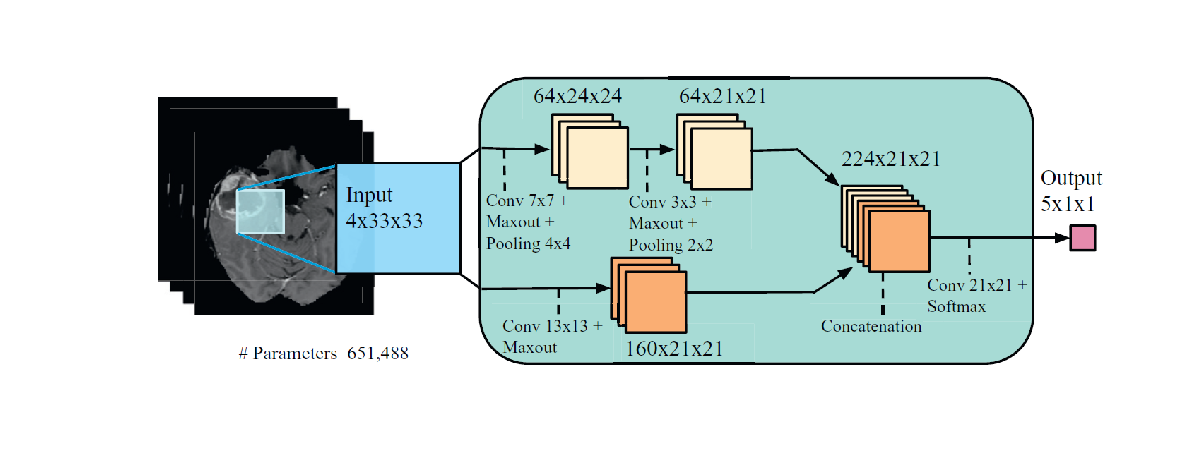
\psfig{file=Two-Pathway.pdf,width =5.3in}
\caption{The base two-pathway architedcture used by Havaei, et al. ~\cite{Havaei:2017}}
\label{fig:twoPathways}
\end{figure*}

The three different cascaded architectures implemented by Havaei, et al. are variations on their two pathway approach described above; both of the CNNs, the original and the one being concatenated in later, use two pathways. The main variation between these three different architectures is the location of the concatenation of the first CNN with the second. Looking at the basic architecture seen in figure~\ref{fig:twoPathways} the first implementation, InputCascadeCNN, takes the output of the first CNN and directly concatenates it to the input of the second CNN. The second implementation, LocalCascadeCNN, takes the output of the first CNN and concatenates it to the first convolutional layer of the second CNNs local pathway. The final implementation, MFCascadeCNN, concatenates the output of the first CNN to the final layer of the second CNN, directly before its output.

The third main component in the research done by Havaei, et al. is their adoption of a two-phase training system. One of the large issues in training CNNs for segmentation is the relative abundance of healthy tissue as compared to the small quantities of tissue that fall under each label. This is especially true of brains where labels can be comprised of less than 1 percent of the total images composition, tumors are likely present on only small amounts of the brain for instance. To alleviate this problem Havaei, et al. first train the CNN on a data set of image patches where all of the labels are equally probable. They then retrain the final output layer taking into account the relative probabilities of the labels,thereby keeping the discriminatory capability of the previous layers intact while maintaining proper output probabilities.



\subsection{3D multi-scale approach in 3 lesion segmentation tasks}
\label{sec:3DMultiScale}

In~\cite{Kamnitsas:2017}, Kamnitsas, et al. provide one of the most recent architectural approaches to CNNs in the field of medical imaging segmentation. Their work can be boiled down to a few main techniques drawing from a wealth of past research. These main techniques include the use of 3D CNNs, dense-inference for network training, 3D CRFs for the final processing of the networks soft segmentation maps, deep networks for better discrimination and two pathways using a multi-scale approach.

Much like the work done by Havaei, et al. Kamnitsas, et al. uses a two pathway approach to better capture local information while maintaining the broader context of the entire image. However, while Havaei, et al. accomplishes this two pathway approach by using a different sized receptive field in each pathway, Kamnitsas, et al. downsamples the image itself.


\begin{figure*}
\centering
\psfig{file=3D CNN.pdf,width =7in}
\caption{The basic neural network architecture used by Kamnitsas, et al. in~\cite{Kamnitsas:2017}}
\label{fig:DeepMedic}
\end{figure*}

The network displayed in figure~\ref{fig:DeepMedic} is a simplified version of Kamnitsas full blown network 'DeepMedic'. As can be seen in the figure the network has two pathways, one with the normal resolution image patch and the other with a down-sampled patch. These patches then go through a series of convolutional layers before two fully connected layers and the final classifier layer. DeepMedic has twice as many convolutional layers as the depicted figure, using a smaller 3\textsuperscript{3} kernel size.

One of the biggest attributes of the work done by Kamnitsas, et al. is the use of 3D CNNs for the basis of their architecture. In the past, research has avoided the use of full blown 3D CNNs due to their increase in parameters and computational requirements.  Hybrid approaches such as training on three orthogonal slices (coronal, sagittal and axial) have been used to cheaply approximate 3D CNNs~\cite{Roth:2014}. The 3D CNNs used by Kamnitsas, et al. use three-dimensional kernels in the convolutional layers to create the feature maps. This can be thought of as a rectangular prism traversing the volume of the image at hand. The use of these 3D CNNs allow for better representation of the volumetric data and allows for the full exploitation of dense-inference. Dense-inference or dense-training, is a process used by Kamnitsas, et al. to help lower the additional computational costs associated with 3D CNNs. When the input image patch is larger than the receptive field of the CNN the CNN's classification layer can convolve across the patch and output multiple predictions rather than the traditional single prediction. The expected cost savings come from decreasing the number of overlapping patches sampled from the test data.


In CNNs it has been shown that deeper networks, networks with more consecutive layers, have greater discriminitive capability due to their additional non-linearities and better defined local optima. While deeper networks have greater discriminitive power it is also true that they have greater computational costs, which is further exaggerated by the use of 3D convolutions. There is also an increase in the number of trainable parameters that is associated with the use of 3D CNNs. To combat these barriers Kamnitsas, et al. replace convolutional layers that have a standard 5\textsuperscript{3} kernal size with multiple layers that use a smaller 3\textsuperscript{3} kernel size. These smaller kernels require fewer parameters and lead to a significant decrease in element-wise multiplications per layer.~\cite{Kamnitsas:2017}

Deeper networks also suffer from being harder to train. As the network becomes deeper it becomes harder to preserve the signal. This is caused by the multiplication of the signals variance as it propagates through each layer. To alleviate this Kamnitsas, et al. initialize their kernel weights to the normal distribution $N(0,\sqrt{2/n\textsuperscript{in}\textsubscript{l}})$ where $n\textsuperscript{in}\textsubscript{l}$ is the number of weights through which a neuron is connected in layer l to the input. They also use a technique called batch normalization to deal with the similar issue of covariate shift, but this is outside of the scope of this paper.

The final contribution from the work of Kamnitsas, et al. that we will discuss is the use of what they call the first fully 3D CRF, conditional random field. CRFs are used in neural networks as a means of taking the predictions from the normal fully-connected layers and giving them the ability to make predictions given the context of the neighboring areas in the image as well. The structure used by Kamnitsas, et al. uses two kernels to better represent the multi-modal images being used. The result is a more rigid segmentation than that provided by the soft segmentation provided by the more traditional output layer.


\section{Results}
\label{sec:results}
In the result reporting, the three values that are important are the dice score, equivalent to an F test, the sensitivity, based on the frequency of false negatives, and specificity, based on the frequency of false positives.

As mentioned before the work done by Havaei, et al. was applied to the BRATS 2013 challenge. They also attempted to use their system on the BRATS 2014 dataset, but were unable to get the system to work due to problems with the dataset itself. For the BRATS 2013 Challenge contenders used an online evaluation tool that provided Dice, specificity and sensitivity scores for the three categories; the complete tumor region, the core tumor region and the enhancing tumor region. As can be seen in figure~\ref{fig:HavaeiResults} their highest scoring network configuration improved on the state of the art in both accuracy and speed.

\begin{figure*}
\centering
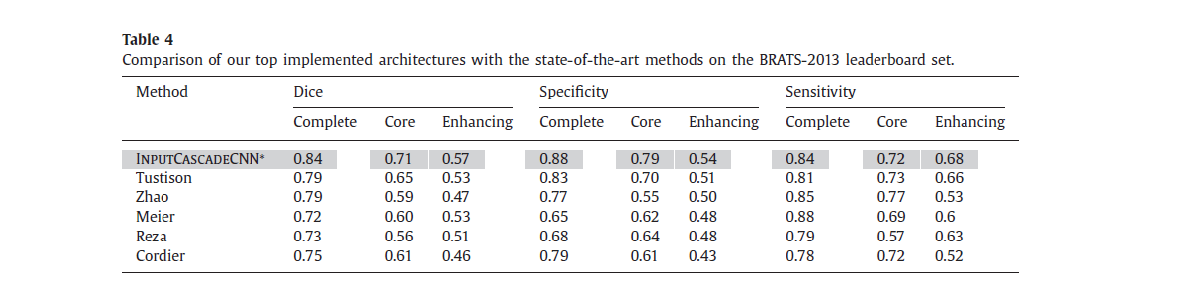
\psfig{file=HavaeiResults.pdf,width =5.3in}
\caption{Havaei, et al. best performnce versus previous state-of-the-arts~\cite{Havaei:2017}.}
\label{fig:HavaeiResults}
\end{figure*}

The architectures proposed by Kamnitsas, et al. were applied to three different brain related challenges. The first was a challenge involving a database of MRIs from people who had suffered traumatic brain injuries, TBI. The second was on the BRATS 2015 dataset, which much like BRATS 2013, measured dice, specificity and sensitivity on the three categories of brain tumor hierarchies, the results can be seen in figure~\ref{fig:KamnitsasResults}. In these results the top score by Ensemble was a combination of three of the DeepMedic neural networks.

The last challenge Kamnitsas, et al. did the ISLES 2015 challenge that dealt with the segmentation of brain lesions caused by stroke. In all cases the DeepMedic + CRF architecture they propose beat the scores of the previous state-of-the-art approaches. Additionally, in all cases the addition of the 3D CRF was found to have a statistically significant effect on performance.

\begin{figure*}
\centering
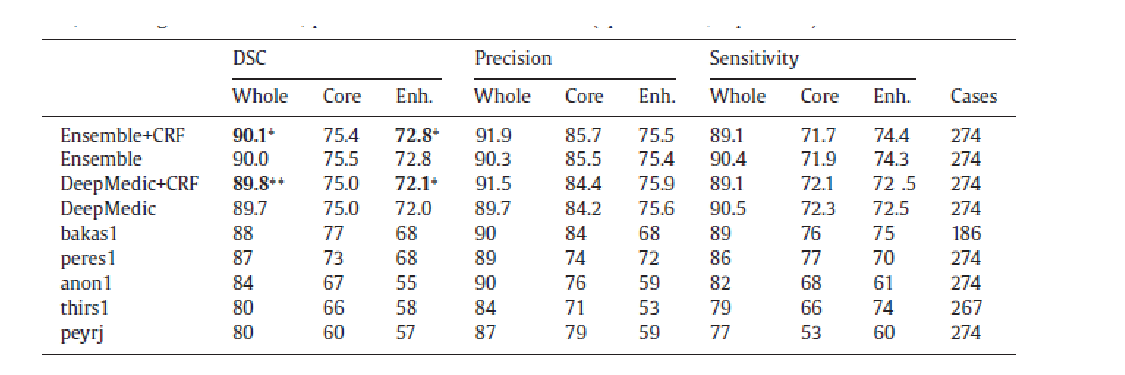
\psfig{file=KamnitsasResults.pdf,width =5.3in}
\caption{Kamnitsas, et al. best performnce versus previous state-of-the-arts(BRATS 2015). The bold numbers indicate a statistically significant difference made by the CRF~\cite{Kamnitsas:2017}.}
\label{fig:KamnitsasResults}
\end{figure*}

\begin{figure}
\centering
\psfig{file=TBI Visuals.pdf,width =4in}
\caption{Three examples from the TBI dataset. The first two columns show the original MRIs with the third column showing the images segmented manually and the last two columns showing the segmentation performed by DeepMedic and DeepMedic with the CRF. Kamnitsas, et al.~\cite{Kamnitsas:2017}}
\label{fig:TBIVisuals}
\end{figure}

Figure ~\ref{fig:TBIVisuals} shows an example pulled from~\cite{Kamnitsas:2017} of DeepMedic's segmentation of three different MRIs. As can be seen in the figure the network does a good job of segmenting both small and large lesions. In the second row however, it undersegments a contusion, possibly mistaking it for background. The third row also shows one of the greater challenges of this segmentation task, where post-surgical sub-dural debris is mistaken as a relevant lesion.~\cite{Kamnitsas:2017}

\section{Conclusions}
\label{sec:conclusions}

As demonstrated by the work of Havaei, et al. and Kamnitsas, et al. convolutional neural networks show a lot of continued promise going forward. The use of multiple pathways for local and global context was shown to be effective in both works. Havaei, et al. has further shown that cascaded architectures with two-phase training are also useful in improving the state-of-the-art. Meanwhile Kamnitsas, et al. have shown that 3D CNNs have become computationally feasible and that Dense-inference and 3D CRFs show promise as well.

These two works are unfortunately not comparable when it comes to the challenges they partook in, but nevertheless both show a breadth of space for further improvement when it comes to CNNs and medical imaging. Future work could combine some of the techniques used such as using a cascaded architecture with DeepMedic or attempting two-phase training.


\section*{Acknowledgments}
\label{sec:acknowledgments}


% The following two commands are all you need in the
% initial runs of your .tex file to
% produce the bibliography for the citations in your paper.
\bibliographystyle{abbrv}
% sample_paper.bib is the name of the BibTex file containing the
% bibliography entries. Note that you *don't* include the .bib ending here.
\bibliography{main}  
% You must have a proper ".bib" file
%  and remember to run:
% latex bibtex latex latex
% to resolve all references

\end{document}
